\subsection{Media Player}
This subsystem is apart of the graphical interface that allows the user to play/stop a song streaming from a third party music service.

\begin{figure}[h!]
	\centering
 	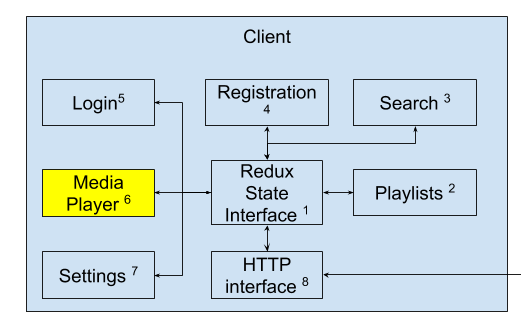
\includegraphics[width=0.60\textwidth]{images/client/client_media.png}
 	\caption{Media player subsystem}
\end{figure}

\subsubsection{Assumptions}
Assuming that the URL's that are sent from the third party music services are valid and are able to be streamed without any geographic restrictions.

\subsubsection{Responsibilities}
The Media Player subsystem is responsible for displaying the albums artwork (if available), and loading and playing/stopping a song from a remote URL from a third party music services. It also displays the remaining time left in the song.

\subsubsection{Subsystem Interfaces}
\begin {table}[H]
\caption {Media player interfaces} 
\begin{center}
    \begin{tabular}{ | p{1cm} | p{6cm} | p{3cm} | p{3cm} |}
    \hline
    ID & Description & Inputs & Outputs \\ \hline
    \#xx & Play song, HTTP request & \pbox{3cm}{Clicking Play} & \pbox{3cm}{Displays Artwork, music plays through user's speakers}  \\ \hline
    \end{tabular}
\end{center}
\end{table}

\newpage